\documentclass[letterpaper,oneside]{book}
%\documentclass[letterpaper,twoside]{book}
% the two-column setup looks better for letter paper with a larger width.
\usepackage{geometry}
\geometry{margin=1.5cm, vmargin={0pt,1cm}}
\setlength{\topmargin}{-1cm}
\setlength{\paperheight}{29.7cm}
\setlength{\textheight}{25.1cm}

% auto adjust the marginals
\usepackage{marginfix}

%\usepackage[algo2e,lined,boxed,linesnumbered]{algorithm2e}

\usepackage{algorithm}
\usepackage{algpseudocode}
\usepackage{subcaption}
\usepackage{graphicx}

\usepackage{amsfonts}
\usepackage{amsmath}
\usepackage{amssymb}
\usepackage{amsthm}
%\usepackage{CJKutf8}
\usepackage{enumerate}
\usepackage{enumitem}
\usepackage{fancyhdr}
\usepackage{graphicx}
\usepackage{caption}
\usepackage{float}
\usepackage{layout}
\usepackage{lineno}
\usepackage{makeidx}
\usepackage{mathrsfs}
\usepackage[version=4]{mhchem}
\usepackage{lipsum}
\usepackage{multicol,caption}
\usepackage{natbib}
%\usepackage{subfigure}
\usepackage{tcolorbox} % this package is needed for \voidenvironment below
\usepackage{tikz}
\usepackage{multirow}
\usetikzlibrary{arrows,automata,backgrounds,cd}
\usetikzlibrary{shapes,snakes}

\newcommand{\Rx}[1]{\mathrm{R}[#1]}
\newcommand{\Lx}[1]{\mathrm{L}[#1]}
\newcommand{\Ux}[1]{\mathrm{U}[#1]}
\newcommand{\Dx}[1]{\mathrm{D}[#1]}
\newcommand{\Cx}[1]{\mathrm{C}[#1]}
\newcommand{\Sx}[1]{\mathrm{S}[#1]}

\newcommand{\ccg}[1]{\overline{#1}}
\newcommand{\dif}{\mathrm{d}}
\newcommand{\Dim}{\mathrm{D}}
\newcommand{\avg}[1]{\left\langle #1 \right\rangle}
\newcommand{\innerProd}[1]{\left\langle #1 \right\rangle}
\newcommand{\cond}{\mathrm{cond}}
\newcommand{\Cond}[2]{\mathrm{cond}_{#1}\left(#2\right)}
\newcommand{\difFrac}[2]{\frac{\dif #1}{\dif #2}}
\newcommand{\gen}[1]{\left\langle #1 \right\rangle}
\newcommand{\ii}{\mathbf{i}}
\newcommand{\Imz}{\mathrm{Im}\,}
\newcommand{\Int}{\mathrm{Int}}
\newcommand{\Ext}{\mathrm{Ext}}
\newcommand{\Cl}{\mathrm{Cl}}
\newcommand{\Fr}{\mathrm{Fr}}
\newcommand{\Ker}{\mathrm{ker}}
\newcommand{\pdfFrac}[2]{\frac{\partial #1}{\partial #2}}
\newcommand{\Rez}{\mathrm{Re}\,}
\newcommand{\sgn}{\mathrm{sgn}}
\newcommand{\Span}{\mathrm{span}}
\newcommand{\OFL}{\mathrm{OFL}}
\newcommand{\UFL}{\mathrm{UFL}}
\newcommand{\fl}{\mathrm{fl}}
%\newcommand{\op}{\mathrm{op}}
\newcommand{\op}{\odot}
\newcommand{\Eabs}{E_{\mathrm{abs}}}
\newcommand{\Erel}{E_{\mathrm{rel}}}
\newcommand{\dom}{\mathrm{dom}}
\newcommand{\Null}{\mathrm{null}}
\newcommand{\Range}{\mathrm{range}}
\newcommand{\Supp}{\mathrm{supp}}
\newcommand{\Arity}{\mathrm{arity}}
\newcommand{\by}[1]{\boldsymbol{#1}}

\newenvironment{Figure}
{\par\medskip\noindent\minipage{\linewidth}}
{\endminipage\par\medskip}

% this environment is for solutions of examples and exercises
\newenvironment{solution}%
{\noindent\textbf{Solution.}}%
{\qedhere}
% the following command is for disabling environments
%  so that their contents do not show up in the pdf.
\makeatletter
\newcommand{\voidenvironment}[1]{%
  \expandafter\providecommand\csname env@#1@save@env\endcsname{}%
  \expandafter\providecommand\csname env@#1@process\endcsname{}%
  \@ifundefined{#1}{}{\RenewEnviron{#1}{}}%
}
\makeatother



%----------------------------------------
% theorem and theorem-like environments %
%----------------------------------------
\numberwithin{equation}{chapter}
\theoremstyle{definition}

\newtheorem{thm}{Theorem}[chapter]
\newtheorem{alg}[thm]{Algorithm}
\newtheorem{asm}[thm]{Assumption}
\newtheorem{axm}[thm]{Axiom}
\newtheorem{coro}[thm]{Corollary}
\newtheorem{defn}[thm]{Definition}
%\newtheorem{exm}{Example}[chapter]
%\newtheorem{exc}[exm]{Exercise}
% number examples and exercises with thms.
\newtheorem{exm}[thm]{Example}
\newtheorem{exc}[thm]{Exercise}
\newtheorem{frm}[thm]{Formula}
\newtheorem{lem}[thm]{Lemma}
\newtheorem{ntn}{Notation}
\newtheorem{prop}[thm]{Proposition}
\newtheorem{rem}{Remark}[chapter]
\newtheorem{rul}[thm]{Rule}



%%%%%%%%%%%%%% for INSE %%%%%%%%%%%%%
\usepackage{bm}
\usepackage[sans]{dsfont}
\usepackage{url}
\newcommand{\ibold}{{\mathbf{i}}}
\newcommand{\jbold}{{\mathbf{j}}}
\newcommand{\kbold}{{\mathbf{k}}}
\newcommand{\ebold}{{\mathbf{e}}}
\newcommand{\ubold}{{\mathbf{u}}}
\newcommand{\xbold}{{\mathbf{x}}}
\newcommand{\pbold}{{\mathbf{p}}}
\newcommand{\etabold}{\bm{\eta}}
\newcommand{\unitV}{\mathds{1}}
\newcommand{\zerobold}{{\mathbf{0}}}
\newcommand{\dt}{{\Delta t}}
\newcommand{\avgI}[1]{\langle #1 \rangle_{\ibold}}
\newcommand{\iphed}{{\ibold+\frac{1}{2}\ebold^d}}
\newcommand{\imhed}{{\ibold-\frac{1}{2}\ebold^d}} %new
% i plus fractional e^d
\newcommand{\ipfed}[1]{\ibold+\frac{#1}{2}\ebold^d}
% i minus fractional e^d
\newcommand{\imfed}[1]{\ibold-\frac{#1}{2}\ebold^d}
\newcommand{\ipmfed}[1]{\ibold\pm\frac{#1}{2}\ebold^d}
\newcommand{\half}{\frac{1}{2}}
\newcommand{\Lapl}{{\mathbf{L}}}
\newcommand{\Div}{{\mathbf{D}}}
\newcommand{\Grad}{{\mathbf{G}}}
\newcommand{\Iden}{{\mathbf{I}}}
\newcommand{\nref}{n_{\text{ref}}}
\newcommand{\phio}{\phi^{\circ}}
\newcommand{\eq}[1]{(\ref{#1})}
\newcommand{\Proj}{{\mathbf{P}}}
\newcommand{\cProj}{{\mathcal{P}}}
\newcommand{\cProjLH}{{\mathscr{P}}}
\newcommand{\ProjAux}{{\mathbf{Q}}}
\newcommand{\exOp}{{\mathbf{X}}^{[\text{E}]}}
\newcommand{\imOp}{{\mathbf{X}}^{[\text{I}]}}
\newcommand{\nStages}{n_{\tiny \textsf{s}}}
\newcommand{\mb}[1]{\mathbf{#1}}
%%%%%%%%%%%%%%%%%%%%%%%%%%%%%%%%%
\newcommand{\fYear}{2025}

\usepackage{ctex}

%\makeindex
  
\begin{document}
\pagenumbering{roman}

%\thispagestyle{empty}
\begin{small}
\tableofcontents
\end{small}

% --------------------------------------------------------
% uncomment the following to remove these environments 
%  to generate handouts for students.
% --------------------------------------------------------
\begingroup
%\voidenvironment{rem}%
%\voidenvironment{proof}%
%\voidenvironment{solution}%
% \input{sec/methodsOfStudy}

%\setcounter{chapter}{-1}
\pagenumbering{arabic}

\setcounter{page}{1}

%\clearpage

% This page has been intentionally left blank.

% \clearpage

\pagestyle{fancy}
\fancyhead{}
\lhead{木子}
\chead{Vision Auto-Regressive Model}
\rhead{\fYear}
\chapter{视觉自回归生成模型}
%\begin{multicols}{2}
%\setlength{\columnseprule}{0.2pt}
% \begin{rem}
%   Based on the universal approximation theorem, the MLPs play a
%   significant role in the field of deep learning.
%\end{rem}
\section{预备知识}
\subsection{VQ-VAE}
自编码器(Auto Encoder, AE)是一种用来提取数据关键特征的自监督模型,它通过将高维的原始数据转化为
低维的潜在特征(latent feature),再利用该特征解码复现原始数据。在图像自编码器模型中,原始图像
通过一个 CNN 或 ViT 编码器模型得到低维潜在特征,再通过类似结构的解码器复现原始图像,损失函数为
AE 模型输入和输出之间的均方误差(重建损失)。

在自编码模型中,其不能生成训练数据集之外的新数据,变分自编码器(Variational Auto Encoder, VAE)
通过假设特征向量服从某种分布规律从而可以从该分布中采样特征向量来生成新的数据。
VAE 假设特征向量服从标准正态分布,编码器输出为均值和方差,解码器通过均值和方差采样重建输入,
损失函数包括重建损失以及特征向量分布与标准正态分布之间的 KL 散度,其中采用重参数化使得
采样过程可导,即:
\begin{equation}
    \bm{z}\sim\mathcal{N}(\bm{\mu},\bm{\sigma}^2)=\bm{\mu}+\bm{\sigma}\cdot\epsilon
    \sim\mathcal{N}(0,1)=g(\epsilon).
\end{equation}

VAE 的潜在空间是连续的,使得生成的样本可能出现过度平滑、难以控制、缺乏足够细节的问题,
VQ (vector quantization)技术通过对特征向量进行量化,通过聚类将连续的潜在空间离散化,
从而高效控制特征的结构和表达分布,VQ-VAE 即是中间表示层为离散值的自编码器。
VQ-VAE 量化模块引入了一个码本(codebook)存储离散的特征向量,每个特征向量有一个一一对应的
索引,对于一个输入图像 $\bm{x}\in\mathbb{R}^{H\times W\times C}$,VQ-VAE 的工作流程如下:
\begin{enumerate}
    \item 通过编码器得到特征图:$\bm{z}_e=E(\bm{x})\in\mathbb{R}^{H\times W\times D}$;
    \item 对于特征图中的每个位置,通过在码本中寻找最近邻,得到 $\bm{z}_q=Q(\bm{z}_e)\in\mathbb{R}^{H\times W\times D}$,
    对于每个 $\bm{z}_q$, 存在一个索引矩阵与之对应;
    \item 最后解码器将 $\bm{z}_q$ 作为输入重建原始图像,记输出为 $\hat{\bm{x}}=G(\bm{z}_q)\in\mathbb{R}^{H\times W\times 3}$。
\end{enumerate}
VQ-VAE 的损失函数包括重建损失以及码本学习损失,其中引入直通梯度估计(STE)来进行梯度传播,具体如下:
\begin{align}
    \mathcal{L}_{VQ-VAE}&=\mathcal{L}_{\text{recon}} + \beta\mathcal{L}_{\text{codebook}} + \gamma\mathcal{L}_{\text{commitment}},\\
    \mathcal{L}_{\text{recon}}&=\|\bm{x}-G(\bm{z}_q)\|_2^2 = \|\bm{x}-G(\bm{z}_e + \text{sg}[\bm{z}_q-\bm{z}_e])\|_2^2,\\
    \mathcal{L}_{\text{codebook}}&=\|\text{sg}[\bm{z}_e]-\bm{z}_q\|_2^2,\\
    \mathcal{L}_{\text{commitment}}&=\|\bm{z}_e-\text{sg}[\bm{z}_q]\|_2^2.
\end{align}
其中 $\text{sg}$ 表示该项不计算梯度。

\subsection{VQ-GAN}

VQGAN 在 VQ-VAE 的基础上,增加了感知损失以及生成对抗损失加以改进模型。
生成对抗模型 GAN 的损失函数为:
$$
\begin{cases}
    \mathcal{L}_G=-\mathbb{E}_{z\sim p_z}[\log (D(G(z)))];\\
    \mathcal{L}_D=-\mathbb{E}_{x\sim p_{\text{data}}}[\log (D(x))]-\mathbb{E}_{z\sim p_z}[\log (1-D(G(z)))].
\end{cases} 
$$
VQGAN 的损失函数包括 VQ-VAE 的损失以及感知损失和生成对抗损失,具体如下:
\begin{equation}
    \mathcal{L}_{VQGAN}=\mathcal{L}_{VQ-VAE}+\alpha\mathcal{L}_{\text{perceptual}}+\lambda\mathcal{L}_{\text{GAN}}.
\end{equation}
其中感知损失表示从抽象的层次感知输入图像和重构图像之间的差异,具体为利用一些预训练好的模型(如 VGG等)提取图像的特征图,计算
特征图之间的距离损失。
\section{ViT-VQGAN}

在 VQ-VAE、VQGAN 等模型的基础上,可以额外训练一个在码本向量空间的自回归模型,从而实现条件到图像的
生成模型,这里以 ViT-VQGAN 为例,ViT-VQGAN 是对 VQGAN 进行了一些改进,包括用基于 Transformer 的
ViT 模型替换所有的 CNN 卷积模型,其训练分为两步:
\begin{enumerate}
    \item \textbf{Stage 1: Image Quantization} 训练基于 ViT 的 VQGAN,对于 $256\times256$ 的图像 $\bm{x}$,
    ViT-VQGAN 将其编码为一个 $32\times32$ 的码本特征图 $\bm{z}_q(\bm{x})$。
    \item \textbf{Stage 2: Vector-quantized Image Modeling} 训练一个 decoder-only 的自回归模型去
    建模 $32\times32=1024$ 图像隐空间 token 序列。
\end{enumerate}

在阶段一的训练中,ViT-VQGAN 引入了 \textbf{Factorized codes} 方法,即添加了一个线性投影层将
编码器的输入投影到维度更小的空间,在该空间中进行 VQ 量化后,再投影回原来的空间从而加速运算,
另外,还对隐空间变量以及码本向量进行了 $L_2$ 正则化,这样使得二者的2范数距离等价于余弦相似度,实验发现可以
提高训练稳定性以及重构质量。在损失函数中,ViT-VQGAN 还加入了 logit-laplace 损失,可以促进码本使用率。

对于阶段二,训练一个自回归 Transformer 模型建模 $32\times32$ 图像隐空间 token 序列(逐排展开得到序列),
即训练损失函数为:
\begin{equation}
    \mathcal{L} = -\mathbb{E}[\log(P(x))],
\end{equation}
其中 $P(x)=\prod_{i=1}^{n}P(x_i|x_1,x_2,\cdots,x_{i-1};\theta)$。

\begin{figure}[htbp]
    \centering 
    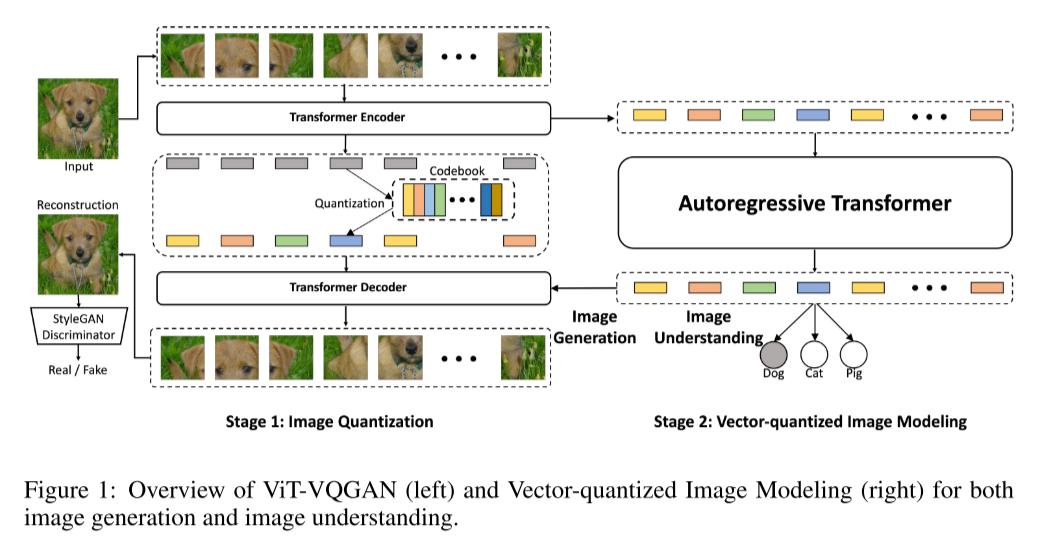
\includegraphics[width=0.8\textwidth]{./fig/ViT-VQGAN.png} 
    %\caption{这是一张示例图片} 
    %\label{fig:example} 
\end{figure}

\section{VAR}

传统的自回归模型基于 next-token 预测,其 token 序列为简单的逐行排列,存在如下问题:
\begin{enumerate}
    \item 数学上的不符。编码器输出的 $\bm{z}_e(\bm{x})$ 其各位置的特征是相互依赖的,即
    $\bm{z}_q(\bm{x})$ 的 token 序列 $(x_1,x_2,\cdots)$ 之间存在双向关系,单向的自回归不适用;
    \item 单向的自回归预测限制了模型的泛化能力,如在双向依赖的问题中;
    \item 逐行排列的自回归结构破坏了图像固有的2D空间结构、依赖关系;
    \item 计算效率低。
\end{enumerate}
VAR 模型提出了基于 next-scale 预测的 multi-scale 自回归新范式,其预测方式符合天然的视觉特性,从模糊到清晰、从结构到细节,
VAR 具有类似于 LLMs 的优良特性:scaling laws 以及 zero-shot generalization;另外,VAR 的出现是自回归模型领域的突破,
在图像生成领域首次超过扩散模型(Diffusion Models)。

不同于 next-token 预测,VAR 基于 next-scale 预测,每个自回归单元为一整个图像 token,而不是单个位置的特征 token,
对于编码器的输出特征 $f\in\mathbb{R}^{h\times w\times C}$,其被量化为 $K$ 个 multi-scale 图像 token 序列
$(r_1,r_2,\cdots,r_K)$,其中分辨率 $h_k\times w_k$ 依次递增,直到 $r_K$ 对应原始大小 $h\times w$,自回归似然函数为:
\begin{equation}
    P(r_1,r_2,\cdots,r_K) = \prod_{k=1}^K P(r_k|r_{1},r_{2},\cdots,r_{k-1}),
\end{equation}
每个自回归单元 $r_k\in[V]^{h_k\times w_k}$,令 $Z$表示码本向量集,$V$表示其大小。在第 $k$ 步预测 $r_k$ 时,
$(r_1,r_2,\cdots,r_{k-1})$作为输入,采用 block-wise 因果注意力掩码。VAR 的这种自回归范式没有破坏图像的空间结构,
并且保持了天然的 $coarse-to-fine$ 的视觉特性,其次,其计算效率也大幅提高。VAR 自回归的具体范式如图~\ref{fig:VAR}所示,多尺度
图像 token 序列 $(r_1,r_2,\cdots,r_K)$ 由如下算法生成,其中 $r_k$ 对应码本中的索引矩阵,$z_k$ 为相应的量化特征向量,
$\hat{f}$ 为基于 $r_k$ 重构的特征向量,算法采用了残差范式,另外为避免扩展 $z_k$ 时的信息丢失,
采用了额外的 $K$ 个卷积层 $\{\phi_k\}_{k=1}^K$ 进行作用。

\begin{figure}[htbp]
    \centering 
    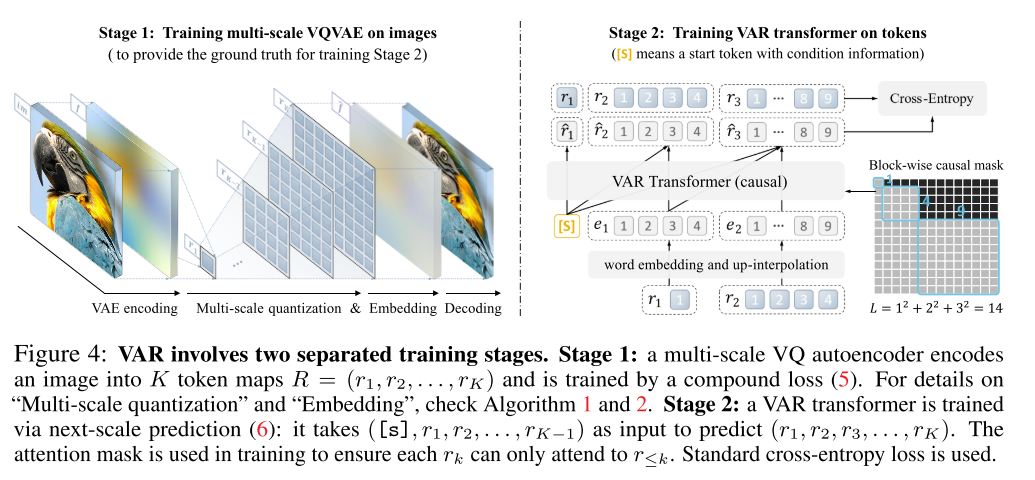
\includegraphics[width=0.8\textwidth]{./fig/VAR.png} 
    %\caption{这是一张示例图片} 
    \label{fig:VAR} 
\end{figure}

% \begin{algorithm}
% \caption{Multi-scale VQVAE Encoding}
% \label{alg:encoding}
% \begin{algorithmic}[1]
% \State Inputs: raw image $im$;
% \State Hyperparameters: steps $K$, resolutions $(h_k, w_k)$ for $k=1$;
% \State $f = E(im)$, $R = []$;
% \For{$k = 1$ to $K$}
%     \State $r_k = Q(\text{interpolate}(f, h_k, w_k))$;
%     \State $R = \text{queue\_push}(R, r_k)$;
%     \State $z_k = \text{lookup}(Z, r_k)$;
%     \State $z_k = \text{interpolate}(z_k, h_K, w_K)$;
%     \State $f = f - \phi_k(z_k)$;
% \EndFor
% \State \Return multi-scale tokens $R$;
% \end{algorithmic}
% \end{algorithm}

% \begin{algorithm}
% \caption{Multi-scale VQVAE Reconstruction}
% \label{alg:reconstruction}
% \begin{algorithmic}[1]
% \State Inputs: multi-scale token maps $R$;
% \State Hyperparameters: steps $K$, resolutions $(h_k, w_k)$ for $k=1$;
% \State $f = 0$;
% \For{$k = 1$ to $K$}
%     \State $r_k = \text{queue\_pop}(R)$;
%     \State $z_k = \text{lookup}(Z, r_k)$;
%     \State $z_k = \text{interpolate}(z_k, h_K, w_K)$;
%     \State $f = f + \phi_k(z_k)$;
% \EndFor
% \State $im = D(f)$;
% \State \Return reconstructed image $im$;
% \end{algorithmic}
% \end{algorithm}

\begin{figure}[htbp]
    \centering
    \begin{minipage}{0.45\textwidth}
        \centering
        \begin{algorithm}[H]
            \caption{Multi-scale VQVAE Encoding}
            \begin{algorithmic}[1]
                \Require raw image $im$; 
                \Require Hyperparameters: steps $K$, resolutions $(h_k, w_k)_{k=1}^K$;
                \State $f = \mathcal{E}(im)$, $R = []$;
                \For{$k = 1, \cdots, K$}
                    \State $r_k = \mathcal{Q}(\text{interpolate}(f, h_k, w_k))$;
                    \State $R = \text{queue\_push}(R, r_k)$;
                    \State $z_k = \text{lookup}(Z, r_k)$;
                    \State $z_k = \text{interpolate}(z_k, h_K, w_K)$;
                    \State $f = f - \phi_k(z_k)$;
                \EndFor
                \Ensure multi-scale tokens $R$;
            \end{algorithmic}
        \end{algorithm}
    \end{minipage}\hfill
    \begin{minipage}{0.45\textwidth}
        \centering
        \begin{algorithm}[H]
            \caption{Multi-scale VQVAE Reconstruction}
            \begin{algorithmic}[1]
                \Require multi-scale token maps $R$;
                \Require Hyperparameters: steps $K$, resolutions $(h_k, w_k)_{k=1}^K$;
                \State $\hat{f} = 0$;
                \For{$k = 1, \cdots, K$}
                    \State $r_k = \text{queue\_pop}(R)$;
                    \State $z_k = \text{lookup}(Z, r_k)$;
                    \State $z_k = \text{interpolate}(z_k, h_K, w_K)$;
                    \State $\hat{f} = \hat{f} + \phi_k(z_k)$;
                \EndFor
                \State $\hat{im} = \mathcal{D}(\hat{f})$;
                \Ensure reconstructed image $\hat{im}$;
            \end{algorithmic}
        \end{algorithm}
    \end{minipage}
    \caption{Algorithms for Multi-scale VQVAE Encoding and Reconstruction}
\end{figure}
\section{Infinity}

基于图像生成模型 VAR,Infinity 是对其进行优化而产生的文生图自回归模型。
VAR 采用传统的 index-wise 离散 tokenizer,受限于码本的词汇量大小,其面临着量化误差以及细节生成等问题,
尤其是对于产生高分辨率的图像,在生成阶段,它还面临着视觉细节丢失、局部扭曲、误差累计等问题。
针对这些问题,Infinity 进行了如下改进:
\begin{enumerate}
    \item \textbf{Bitwise visual tokenizer.} 采用 binary vector quantization 技术,将码本词汇量提升至
    $2^{64}$,因此显著提高了图像生成质量;
    \item \textbf{Bitwise infinite-vocabulary classfier.} 采用基于 binary bit 的分类预测,不同于传统的
    分类模型,在如此大码本下仍能保持高效的运算和优化;
    \item \textbf{Bitwise self-correction.} 在训练阶段随机 flip some bits 模拟预测错误,并重新量化残差特征,
    即随机引入预测误差,但在此误差下仍预测正确的残差特征,从而使模型获得自我纠正的能力。 
\end{enumerate}
Infinity 即是 bitwise VAR,它保持了 VAR 的 scaling 以及 speed 优势,同时也解决了 VAR 面临的问题,能够
实现高质量的图像生成效果,超过了 SD3-Medium 等扩散模型。

\subsection{Visual AutoRegressive Modeling}
Infinity 架构包括一个 visual tokenizer 以及 用于文生图的自回归 Transformer 模型,对于数据对
(prompt text $t$,image $I$),类似于 VAR, $I$ 首先被编码为特征 $F\in\mathbb{R}^{h\times w\times d}$,
然后量化得到 $K$ 个 multi-scale 残差特征 $(R_1, R_2, \cdots, R_K)$,定义
\begin{equation}
    F_k = \sum_{i=1}^{k} \text{upsample}(R_i,(h,w)),
\end{equation}
$F_k$ 逐渐逼近原始特征 $F$。自回归似然函数为
\begin{equation}
    P(R_1,\cdots,R_K) = \prod_{k=1}^K P(R_k|R_1,\cdots,R_{k-1},\Psi(t)),
\end{equation}
其中 $\Psi(t)$ 为基于 Flan-T5 模型的文本编码,在输入端,$\Psi(t)$ 首先被投影为一个 <SOS> token 作为第一步输入,
之后,每个 tranformer block,$\Psi(t)$ 还通过交叉注意力引导图像生成,在第 $k$ 步预测 $R_k$ 时,
$(\Psi(t),R_1,\cdots,R_{k-1})$ 作为输入,实际训练中,为匹配每一步输入输出端的分辨率大小,引入
\begin{equation}
    \tilde{F}_{k-1} = \text{downsample}(F_{k-1},(h_k,w_k)),
\end{equation}
作为输入去预测 $R_k$,故在第 $k$ 步预测中,实际的输入为 $(<SOS>,\tilde{F}_1,\cdots,\tilde{F}_{k-1})$,
$\tilde{F}_{k-1}$ 的分辨率大小与 $R_k$ 相同,在 VAR 中利用 $R_{k-1}$ 预测 $R_k$,输入时 $R_{k-1}$ 首先
经过了上采样以匹配 $R_k$ 的分辨率大小,相比之下 Infinity 处理方式更为恰当。

\begin{figure}[htbp]
    \centering 
    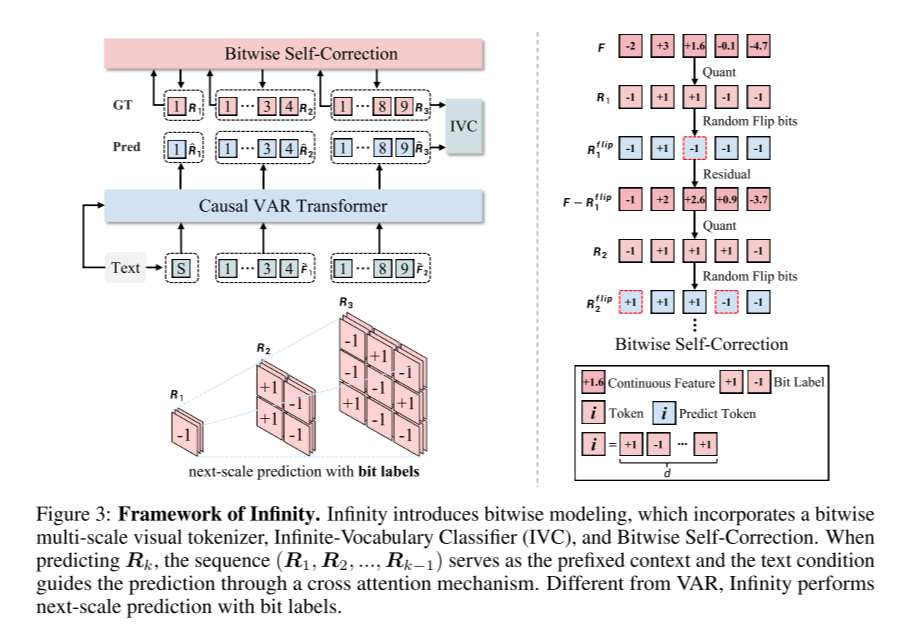
\includegraphics[width=0.8\textwidth]{./fig/Framework of Infinity.png} 
    %\caption{这是一张示例图片} 
    %\label{fig:example} 
\end{figure}

\subsection{Bitwise Visual Tokenizer}
增加码本的词汇量大小会显著增加存储和计算开销,为解决这个问题,Infinity 采用了 Bitwise multi-scale residual quantizer,
对每个尺度的特征向量 $z_k\in\mathbb{R}^d$,其被量化为 binary output $q_k$,
\begin{equation}
    q_k = Q(z_k) = \begin{cases}
        \text{sign}(z_k)\quad\text{if LFQ};\\
        \frac{1}{\sqrt{d}}\text{sign}(\frac{z_k}{|z_k|})\quad\text{if BSQ}.
    \end{cases}
\end{equation}
另外引入熵惩罚项 $\mathcal{L}_{\text{entropy}}=\mathbb{E}[H(q(z))]-H(\mathbb{E}[q(z)])$ 用于增加码本的利用率。

\subsection{Bitwise Infinite-Vocabulary Classifier}
由于码本词汇量巨大,在预测 $R_k$ 时,若采用原始的 softmax 分类器,会导致巨大的计算量,Infinity 采用 d 个二元分类器同时预测
$R_k$ 的每个 bit 是正还是负,从而大大提高效率和预测的鲁棒性。

\begin{figure}[htbp]
    \centering 
    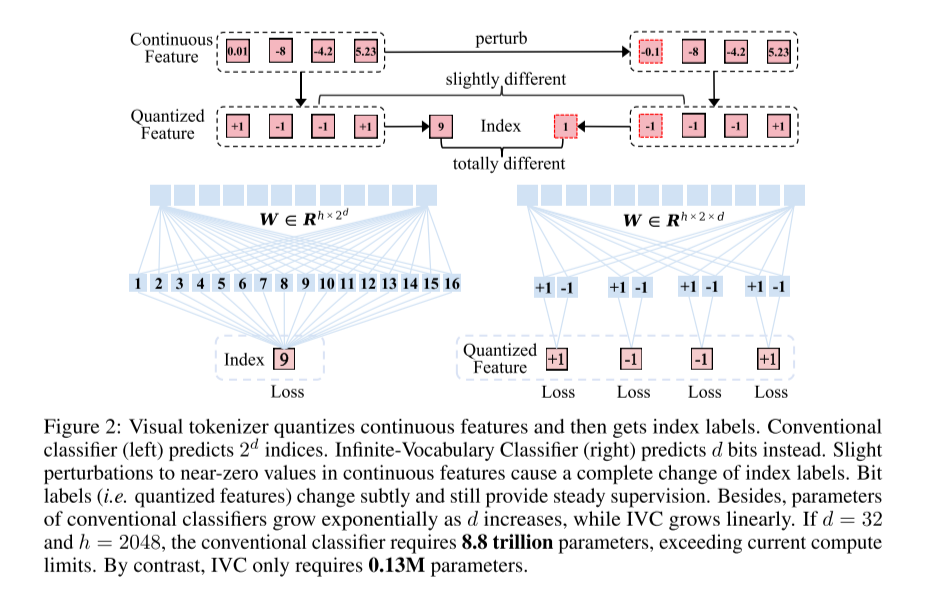
\includegraphics[width=0.8\textwidth]{./fig/IVC.png} 
    %\caption{这是一张示例图片} 
    %\label{fig:example} 
\end{figure}
\subsection{Bitwise Self-Correction}
在训练阶段,每一步的预测均是细化之前的输出,增加细节,但在实际生成过程中,若中间某一层出现预测误差时,模型
缺乏识别并修正错误的能力,从而导致误差累计。Infinity 根据一定概率随机 flip some bits 模拟预测错误,并重新量化残差特征,
这种引入过程错误,并根据错误调整预测目标使得模型具有识别并纠正错误的能力。

\begin{figure}[htbp]
    \centering
    \begin{minipage}{0.45\textwidth}
        \centering
        \begin{algorithm}[H]
            \caption{Visual Tokenizer Encoding}
            \begin{algorithmic}[1]
                \Require raw feature $F$, scale schedule $\{(h_1^r, w_1^r), ..., (h_K^r, w_K^r)\}$
                \State $R_{\text{queue}} = []$ \Comment{multi-scale bit labels}
                \State $\tilde{F}_{\text{queue}} = []$ \Comment{inputs for transformer}
                \For{$k = 1, 2, \cdots, K$}
                    \State $R_k = \mathcal{Q}(\text{down}(F - F_{k-1}, (h_k, w_k)))$
                    \State $\text{Queue\_Push}(R_{\text{queue}}, R_k)$
                    \State $F_k = \sum_{i=1}^{k} \text{up}(R_i, (h, w))$
                    \State $\tilde{F}_k = \text{down}(F_k, (h_{k+1}, w_{k+1}))$
                    \State $\text{Queue\_Push}(\tilde{F}_{\text{queue}}, \tilde{F}_k)$
                \EndFor
                \Ensure $\tilde{R}_{\text{queue}}, \tilde{F}_{\text{queue}}$
            \end{algorithmic}
        \end{algorithm}
    \end{minipage}\hfill
    \begin{minipage}{0.45\textwidth}
        \centering
        \begin{algorithm}[H]
            \caption{Encoding with BSC}
            \begin{algorithmic}[1]
                \Require raw feature $F$, random flip ratio $p$, scale schedule $\{(h_1^r, w_1^r), ..., (h_K^r, w_K^r)\}$
                \State $R_{\text{queue}} = [], \tilde{F}_{\text{queue}} = []$
                \For{$k = 1, 2, \cdots, K$}
                    \State $R_k = \mathcal{Q}(\text{down}(F - F_{k-1}^{\text{flip}}, (h_k, w_k)))$
                    \State $\text{Queue\_Push}(R_{\text{queue}}, R_k)$
                    \State $R_k^{\text{flip}} = \text{Random\_Flip}(R_k, p)$
                    \State $F_k^{\text{flip}} = \sum_{i=1}^{k} \text{up}(R_i^{\text{flip}}, (h, w))$
                    \State $\tilde{F}_k = \text{down}(F_k^{\text{flip}}, (h_{k+1}, w_{k+1}))$
                    \State $\text{Queue\_Push}(\tilde{F}_{\text{queue}}, \tilde{F}_k)$
                \EndFor
                \Ensure $R_{\text{queue}}, \tilde{F}_{\text{queue}}$
            \end{algorithmic}
        \end{algorithm}
    \end{minipage}
    \caption{Algorithms for Visual Tokenizer Encoding and Encoding with BSC}
\end{figure}

\clearpage
%\chapter{The Kolmogorov-Arnold Networks (KANs)}
%\label{chapter:KANs}
% \begin{rem}
%   Recently,
%   a promising alternative representation model, KANs, 
%   which are based the Kolmogorov-Arnold representation theorem,
%   were proposed by Liu et al\cite{liu2024kan}.
% \end{rem}
%\input{sec/KAN}

%\clearpage
%\chapter{The Comparison between MLP and KAN Representations for Differential Equations and Operator Networks}
%\input{sec/ComparisonOnPDE}
%\end{multicols}



\clearpage

\pagestyle{fancy}
\fancyhead{}
\lhead{}
\chead{Bibliography}
\rhead{\fYear}

\bibliography{bib/ref}
%\bibliographystyle{abbrv}
\bibliographystyle{abbrvnat}
\setcitestyle{author,year,open={[},close={]}}
\nocite{*}
\printindex

\end{document}



%%% Local Variables: 
%%% mode: latex
%%% TeX-master: t
%%% End: 

% LocalWords:  FPN underflows denormalized FPNs matlab eps IEEE iff
% LocalWords:  cardinality significand quadratically bijection unary
%  LocalWords:  contractive bijective postcondition invertible arity
%  LocalWords:  subspaces surjective injective monomials additivity
%  LocalWords:  nullary Abelian abelian finitary eigenvectors adjoint
%  LocalWords:  eigenvector nullspace Hermitian unitarily multiset
%  LocalWords:  nonsingular nonconstant homomorphism homomorphisms
%  LocalWords:  isomorphically indeterminates subfield isomorphism
%  LocalWords:  nondefective diagonalizable contrapositive cofactor
%  LocalWords:  submatrix nilpotent positivity orthonormal extremum
%  LocalWords:  Jacobian nonsquare semidefinite nonnegative RHS LLS
%  LocalWords:  roundoff
